\begin{answer}

    \begin{figure*}[h]
        \centering
        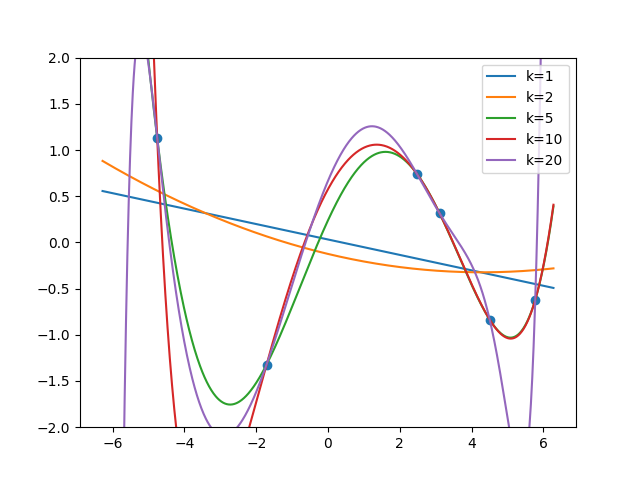
\includegraphics[width=0.6\linewidth]{tex/featuremaps/plot_e.png}
        \caption{Plot of over-fitting}
        \label{fig:my_label}
    \end{figure*}
    
    As the k increases, the hypothesis curve fits well into the training data. However, when the k is over 10, the hypothesis curve acts overly in order to fit the training data. For instance, when the k = 10, 20, the hypothesis curve has huge fluctuation, and even when k is 20, it does not pass one training data. 

\end{answer}
